% --- Template for thesis / report with tktltiki2 class ---
% 
% last updated 2013/02/15 for tkltiki2 v1.02

\documentclass[finnish, grading]{tktltiki2}

% tktltiki2 automatically loads babel, so you can simply
% give the language parameter (e.g. finnish, swedish, english, british) as
% a parameter for the class: \documentclass[finnish]{tktltiki2}.
% The information on title and abstract is generated automatically depending on
% the language, see below if you need to change any of these manually.
% 
% Class options:
% - grading                 -- Print labels for grading information on the front page.
% - disablelastpagecounter  -- Disables the automatic generation of page number information
%                              in the abstract. See also \numberofpagesinformation{} command below.
%
% The class also respects the following options of article class:
%   10pt, 11pt, 12pt, final, draft, oneside, twoside,
%   openright, openany, onecolumn, twocolumn, leqno, fleqn
%
% The default font size is 11pt. The paper size used is A4, other sizes are not supported.
%
% rubber: module pdftex

% --- General packages ---

\usepackage[utf8]{inputenc}
\usepackage[T1]{fontenc}
\usepackage{lmodern}
\usepackage{microtype}
\usepackage{amsfonts,amsmath,amssymb,amsthm,booktabs,color,enumitem,graphicx}
\usepackage[pdftex,hidelinks]{hyperref}
\usepackage{multirow}
\usepackage{tabulary}
\usepackage{float}
\usepackage{enumitem}
%\usepackage{paralist}
\usepackage{listings}

\definecolor{dkgreen}{rgb}{0,0.6,0}
\definecolor{gray}{rgb}{0.5,0.5,0.5}
\definecolor{mauve}{rgb}{0.58,0,0.82}

\lstset{frame=tb,
  language=Java,
  aboveskip=3mm,
  belowskip=3mm,
  showstringspaces=false,
  columns=flexible,
  basicstyle={\small\ttfamily},
  numbers=none,
  numberstyle=\tiny\color{gray},
  keywordstyle=\color{blue},
  commentstyle=\color{dkgreen},
  stringstyle=\color{mauve},
  breaklines=true,
  breakatwhitespace=true,
  tabsize=3
}

\hyphenation{luok-ka-mu-taa-ti-o-o-pe-raat-to-ri}

% Automatically set the PDF metadata fields
\makeatletter
\AtBeginDocument{\hypersetup{pdftitle = {\@title}, pdfauthor = {\@author}}}
\makeatother

% References ilman bracket

\makeatletter 
\renewcommand\@biblabel[1]{#1} 
\makeatother

% --- Language-related settings ---
%
% these should be modified according to your language

% babelbib for non-english bibliography using bibtex
\usepackage[fixlanguage]{babelbib}
\selectbiblanguage{finnish}

% add bibliography to the table of contents
\usepackage[nottoc]{tocbibind}
% tocbibind renames the bibliography, use the following to change it back
\settocbibname{Lähteet}

% --- Theorem environment definitions ---

\newtheorem{lau}{Lause}
\newtheorem{lem}[lau]{Lemma}
\newtheorem{kor}[lau]{Korollaari}

\theoremstyle{definition}
\newtheorem{maar}[lau]{Määritelmä}
\newtheorem{ong}{Ongelma}
\newtheorem{alg}[lau]{Algoritmi}
\newtheorem{esim}[lau]{Esimerkki}

\theoremstyle{remark}
\newtheorem*{huom}{Huomautus}


% --- tktltiki2 options ---
%
% The following commands define the information used to generate title and
% abstract pages. The following entries should be always specified:

\title{Mutaatiotestaus oliojärjestelmissä}
\author{Eveliina Pakarinen}
\date{\today}
\level{Tutkielma}
\abstract{Olioperustaisen ohjelmoinnin kehityksen myötä testausmenetelmiä on sopeutettu uusiin vaatimuksiin, joita olio-ohjelmoinnin erityispiirteet ovat tuoneet mukanaan. Mutaatiotestaus on virheperustainen testausmenetelmä, jonka avulla ohjelmiston olemassa olevien testien laatua voidaan kehittää ja parantaa. Mutaatiotestaus esiteltiin ensimmäistä kertaa jo 1970-luvulla.

Perinteisesti mutaatiotestausta on käytetty testien kehittämisessä proseduraalisella ohjelmoinnilla tuotetuille ohjelmille. Olioperustaisten ohjelmien mutaatiotestaukseen on kuitenkin kehitetty luokkamutaatioksi kutsuttu mutaatiotestausmenetelmä. Mutaatiotestaukseen liittyy ratkaisemattomia ongelmia, jotka estävät mutaatiotestauksen laajamittaisen käytön osana ohjelmistotestausta. 
\vspace{1\baselineskip}\vspace{-\parskip}\\ACM Computing Classification System (CCS):
\\D.2.4 [Software/Program Verification]
\\D.2.5 [Testing and Debugging]
\\D.3.3 [Language Constructs and Features]}

% The following can be used to specify keywords and classification of the paper:

\keywords{mutaatiotestaus, oliojärjestelmät, Java}

% classification according to ACM Computing Classification System (http://www.acm.org/about/class/)
% This is probably mostly relevant for computer scientists
% uncomment the following; contents of \classification will be printed under the abstract with a title
% "ACM Computing Classification System (CCS):"
% \classification{D.2.4 [Software/Program Verification]
%\\D.2.5 [Testing and Debugging]
%\\D.3.3 [Language Constructs and Features]}

% If the automatic page number counting is not working as desired in your case,
% uncomment the following to manually set the number of pages displayed in the abstract page:
%
% \numberofpagesinformation{16 sivua + 10 sivua liitteissä}
%
% If you are not a computer scientist, you will want to uncomment the following by hand and specify
% your department, faculty and subject by hand:
%
% \faculty{Matemaattis-luonnontieteellinen}
% \department{Tietojenkäsittelytieteen laitos}
% \subject{Tietojenkäsittelytiede}
%
% If you are not from the University of Helsinki, then you will most likely want to set these also:
%
% \university{Helsingin Yliopisto}
% \universitylong{HELSINGIN YLIOPISTO --- HELSINGFORS UNIVERSITET --- UNIVERSITY OF HELSINKI} % displayed on the top of the abstract page
% \city{Helsinki}
%


\begin{document}

% --- Front matter ---

\frontmatter      % roman page numbering for front matter

\maketitle        % title page
\makeabstract     % abstract page

\tableofcontents  % table of contents

% --- Main matter ---

\mainmatter       % clear page, start arabic page numbering

% Write some science here.

% Tähän tekstiä. \\ Esimerkki lähdeviitteestä: ~\cite{toinen}.

%\[\frac{a}{b}\]

\section{Johdanto}

Perinteisiä ohjelmistojen testausmenetelmiä on olioperustaisen ohjelmoinnin kehityksen myötä sopeutettu uusiin olio-ohjelmoinnin mukana tuleviin haasteisiin. Olio-ohjelmoinnin avulla voidaan ratkaista joitakin proseduraalisen ohjelmoinnin ongelmia~\cite[s. 86]{Mariani:Pezze:2008}. Olio-ohjelmoinnin piirteet, kuten kapselointi ja perintä, aiheuttavat kuitenkin uusia ongelmia.

Ohjelmistokehitysprosessissa testausta voidaan käyttää ohjelmistossa olevien vikojen havaitsemiseen jo kehitysvaiheen aikana. Testauksen avulla voidaan myös parantaa ohjelmiston laatua ja varmistaa, että ohjelma toimii sille asetettujen vaatimusten mukaisesti. 

Testaukseen liittyy kuitenkin myös rajoituksia. Testauksen avulla ei esimerkiksi voi aina todistaa ohjelmiston oikeellisuutta~\cite[s. 58]{Binder:1999}. Lisäksi epävarmuutta liittyy käytettävän testausjärjestelmän oikeellisuuden ja luotettavuuden varmistamiseen.

Yksi menetelmä ohjelmiston testien laadun tutkimiseen ja parantamiseen on mutaatiotestauksen käyttö osana ohjelmiston testausprosessia. Mutaatiotestauksessa tavoitteena on tutkia, ovatko ohjelmistoa varten tehdyt testit laadukkaita ja havaitaanko niillä kattavasti ohjelmistossa mahdollisesti esiintyviä vikoja ja ongelmia~\cite[s. 649]{Jia:Harman:2011}. 

Mutaatiotestauksen periaatteena on simuloida ohjelmoijien tekemiä yleisiä ohjelmointivirheitä muokkaamalla ohjelmiston alkuperäistä lähdekoodia~\cite[s. 649]{Jia:Harman:2011}. Mutaatiotestauksessa lähdekoodista muodostetaan muunnettuja versioita eli mutantteja. 

Perinteisesti mutaatiotestausta on käytetty testien kehityksessä proseduraalisella ohjelmoinnilla tuotetuille ohjelmille. Olioperustaisen ohjelmoinnin kehittyessä mutaatiotestausta on sopeutettu uusiin vaatimuksiin. Luokkamutaation avulla mutaatiotestausta voidaan soveltaa olio-ohjelmia testaavien testien laadun varmistamiseen~\cite{Kim:Clark:McDermid:2000}.

Vaikka mutaatiotestausta voidaan käyttää apuna ohjelmiston olemassa olevien testien kehittämisessä, liittyy mutaatiotestausmenetelmän käyttöön myös ratkaisemattomia ongelmia, jotka estävät mutaatiotestauksen laaja-alaisen käytön~\cite[s. 652]{Jia:Harman:2011}. Mutaatiotestauksen suoritus vaatii paljon laskentatehoa, mikä on yksi ongelmista. Lisäksi mutaatiotestausprosessissa ihmiseltä vaadittava työpanos on suuri. 

Mutaatiotestausta on tutkittu paljon~\cite[s. 649]{Jia:Harman:2011}. Tutkimuksen avulla on etsitty keinoja ratkaista mutaatiotestaukseen liittyviä ongelmia, jotta mutaatiotestaus voidaan muuttaa käytännölliseksi testausmenetelmäksi. 

%\textcolor{cyan}{Tutkimuskysymys: On tutkittu, että mutaatiotestauksesta on hyötyä testien laadun parantamisessa ja testikattavuuden tarkastelussa/kasvattamisessa. Miksi mutaatiotestausta ei kuitenkaan käytetä laajasti näiden asioiden tekemiseen?}
%
%\textcolor{red}{Vastaus: Koska mutaatiotestaus on tällä hetkellä vielä työlästä ja tehotonta sen tuomaan hyötyyn nähden. Koska mutaatiotestauksessa on ratkaisemattomia ongelmia (esim. ekvivalentit mutantit), joita ei voi automatisoida --> vaativat ihmisten panostusta --> lisää työläyttä.} 
%
%\textcolor{blue}{Tai toisinpäin: Miksi mutaatiotestausta käytettäisiin/pitäisi käyttää enemmän testaamiseen, vaikka mutaatiotestaus on tehotonta/työlästä?}
%
%\textcolor{red}{Vastaus: Koska mutaatiotestausta voidaan käyttää testien laadun parantamiseen tai testikattavuuden kasvattamiseen. Koska mutaatiotestauksen avulla voi varmistaa, että testien laatu on hyvä ja näin ollen parantaa samalla ohjelmiston laatua --> ohjelmistosta saadaan suurin osa ongelmista ja virheistä pois testien avulla. Koska mutaatiotestauksella voi paikata normaaliin testaukseen jääneitä puutteita.} 

%Ohjelmistoja voidaan testata monella tasolla. Testauksen tasot muodostetaan määrittämällä joukko ohjelman osia eli komponentteja, joita halutaan testata. Alimmalla testauksen tasolla testattavat ohjelman osat ovat pienimpiä mahdollisia suoritettavissa olevia komponentteja. Tämän tason testausta kutsutaan \textit{yksikkötestaukseksi} (\textit{unit testing}) ja testattavat osat ovat olio-ohjelmissa esimerkiksi yksittäisiä metodeja tai luokkia~\cite[s. 45]{Binder:1999}.
%
%Yksikkötestauksesta seuraava taso ylöspäin on \textit{integraatiotestaus} (\textit{integration testing}), jossa tarkastellaan järjestelmän tai sen osien yhteistoimintaa ja keskinäistä kommunikointia testaamalla osien välisiä rajapintoja. Olio-ohjelmissa luokkien muodostuminen perinnän avulla ja luokkien koostuminen toisten luokkien olioista aiheuttaa sen, että integraatiotestaukselle on tarvetta jo olioperustaisen ohjelmoinnin alkuvaiheessa~\cite[s. 45]{Binder:1999}.
%
%Valmista integroitua sovellusta testataan \textit{järjestelmätestauksen} (\textit{system testing}) avulla. Tällä testauksen tasolla keskitytään vain valmiissa sovelluksessa esiintyvien piirteiden testaamiseen. Testauksen kohteena voi olla esimerkiksi sovelluksen toiminnallisuus, suorituskyky tai sovelluksen kestämä kuormitus~\cite[s. 45]{Binder:1999}.
%
%Testien suunnittelussa ja kehittämisessä voidaan myös käyttää erilaisia suunnittelumalleja, joiden avulla kuvataan testien suunnitteluun käytettävää näkökulmaa. Ohjelman sisäiseen rakenteeseen eli lähdekoodin tuntemukseen perustuvaa testien suunnittelumallia kutsutaan \textit{white box -testaukseksi}. \textit{Black box -testaukseksi} tai \textit{funktionaaliseksi testaukseksi} kutsutussa suunnittelumallissa testejä suunnitellaan analysoimalla ohjelmiston ulkoista toiminnallisuutta~\cite[s. 52]{Binder:1999}.

%Mutanttien generoinnin jälkeen ohjelmiston alkuperäiset testit suoritetaan jokaisen mutantin kohdalla. Tavoitteena on, että testien avulla havaitaan lähdekoodiin tehdyt muutokset. Jos alkuperäiset testit eivät mene läpi, se tarkoittaa, että mutantti on tapettu eli lähdekoodiin tehdyt muutokset on havaittu~\cite[s. 9]{Kim:Clark:McDermid:2000}. 
%
%Mutaatiotestausprosessi tuottaa lopputuloksena \textit{mutaatiopistemäärän} (\textit{mutation adequacy score}), jonka avulla voidaan arvioida ohjelmiston testien laadukkuutta ja kykyä havaita lähdekoodissa olevia vikoja. 


%\textbf{Johdanto jäsennelty asianmukaisesti (kenelle, miksi, millaisessa ympäristössä; ratkaisun lähestymistapa; tutkimuskysymys, tulokset ja impakti), pituus 1,5 - 2 s.}

%\textbf{\textit{MIKÄ ON MINUN TUTKIMUSKYSYMYKSENI?}}


\section{Testaus oliojärjestelmissä}

Olioperustaisen ohjelmoinnin kehityksen myötä klassisia ohjelmistojen testausmenetelmiä on sopeutettu mahdollistamaan \textit{oliojärjestelmien} (\textit{object oriented systems}) kattava ja laadukas testaaminen. Vaikka olioperustainen ohjelmointi ratkaisee joitakin proseduraalisen ohjelmoinnin suunnittelu- ja toteutusongelmia, olio-ohjelmoinnin mukana tulevat uudet haasteet vaativat uusien testaus- ja analysointimenetelmien kehittämistä~\cite[s. 86]{Mariani:Pezze:2008}. 

\subsection{Rooli}

IEEE:n standardin mukaan ohjelmointivirheen (\textit{error}) aiheuttamaa, ohjelmiston lähdekoodiin päässyttä virheellistä kohtaa kutsutaan viaksi (\textit{fault})~\cite[s. 5]{IEEE:2009}. Lähdekoodissa oleva vika saattaa ohjelman suoritusaikana ilmetä virheenä (\textit{failure}). Virhe ilmenee, kun ohjelma ei suorituksen aikana toimi odotetulla tavalla. \textbf{(Tässä tutkielmassa käytetään IEEE:n standardin mukaisia määritelmiä vialle ja virheelle.)}

Testausta käytetään ohjelmistokehityksessä ohjelmiston laadun varmistamiseen ja auttamaan lähdekoodissa esiintyvien vikojen havaitsemisessa jo kehitysvaiheen aikana. Ohjelmistojen testaamisen ensisijainen tavoite on siis paljastaa vikoja, joiden havaitseminen muiden laadunvarmistusmenetelmien avulla olisi työlästä tai mahdotonta~\cite[s. 59]{Binder:1999}. Testauksen avulla pyritään myös varmistamaan, että ohjelma toimii sille asetettujen vaatimusten mukaisesti. %\textit{\textbf{The primary role of software testing is to reveal bugs that would be too costly or impossible to find with other verification and validation techniques. A secondary purpose is to show that the system under test complies with its stated requirements for a given test suite.}}

Olio-ohjelmoinnissa testaukseen tuovat haasteita olio-ohjelmien erityispiirteet, joita ovat muun muuassa kapselointi, perintä, dynaaminen sidonta ja polymorfismi~\cite[s. 86]{Mariani:Pezze:2008}. 

\subsection{Tasot}

Ohjelmistoja voidaan testata usealla tasolla. Testauksen tasoja ovat yksikkö-, integraatio- ja järjestelmätasot. Tasot muodostuvat yhdestä tai useammasta ohjelman komponentista, joita tason testeillä testataan~\cite[s. 45]{Binder:1999}. Komponentti voi olio-ohjelmissa olla esimerkiksi yksittäinen metodi tai luokka, ohjelman luokkien välinen rajapinta tai jo valmis ohjelmisto.

Alimmalla testauksen tasolla \textit{yksikkötestauksessa} (\textit{unit testing}) testataan ohjelman pienimpiä suoritettavissa olevia komponentteja~\cite[s. 45]{Binder:1999}. Olio-ohjelmissa näitä komponentteja ovat yksittäiset metodit ja oliot.

Yksikkötestauksesta seuraava taso ylöspäin on \textit{integraatiotestaus} (\textit{integration testing}), jossa tarkastellaan järjestelmän tai sen osien yhteistoimintaa~\cite[s. 45]{Binder:1999}. Integraatiotestauksessa testataan siis järjestelmän osien välisiä rajapintoja ja osien keskinäistä kommunikointia. Olio-ohjelmissa luokkien muodostumisesta perinnän avulla ja luokkien koostumisesta toisten luokkien olioista seuraa, että integraatiotestaukselle on olio-ohjelmoinnissa tarvetta jo ohjelmoinnin alkuvaiheessa.

Valmista integroitua sovellusta testataan \textit{järjestelmätestauksen} (\textit{system testing}) avulla~\cite[s. 45]{Binder:1999}. Tällä testauksen tasolla keskitytään vain valmiissa sovelluksessa esiintyvien piirteiden testaamiseen. Testauksen kohteena voi olla esimerkiksi sovelluksen toiminnallisuus, suorituskyky tai sovelluksen kestämä kuormitus~\cite[s. 45]{Binder:1999}.

\subsection{Suunnittelu}

Testien suunnitteluun ja kehittämiseen voidaan käyttää useita menetelmiä. Testausmenetelmän avulla kuvataan näkökulmaa, josta esimerkiksi ohjelman lähdekoodia tarkastellaan testejä kehitettäessä~\cite[s. 51]{Binder:1999}. Ohjelman sisäisen rakenteen tai ulkoisen toiminnallisuuden tuntemusta voidaan käyttää testausmenetelmissä apuna uusia testejä kehitettäessä. Lisäksi olemassa olevia testejä voidaan kehittää testausmenetelmien avulla.

Ohjelman sisäisen rakenteen eli lähdekoodin tuntemukseen perustuvaa testausmenetelmää kutsutaan \textit{white box -testaukseksi}~\cite[s. 52]{Binder:1999}. White box -testausta voidaan käyttää esimerkiksi yksikkötestauksessa apuna testien suunnittelussa, sillä lähdekoodin tuntemus auttaa kehittämään testejä yksittäisille metodeille ja olioille.

\textit{Black box -testaukseksi} eli \textit{funktionaaliseksi testaukseksi} kutsutussa testausmenetelmässä testejä suunnitellaan ohjelmiston toiminnallisuuden tuntemuksen avulla~\cite[s. 52]{Binder:1999}. Koska valmiin sovelluksen piirteitä testattaessa tutkitaan myös sovelluksen ulkoista toiminnallisuutta, on black box -testausmenetelmästä apua suunniteltaessa testejä esimerkiksi järjestelmätestaukseen.

\textit{Gray box -} eli \textit{hybriditestauksessa} yhdistetään white box - ja black box -testausmenetelmien piirteitä~\cite[s. 52]{Binder:1999}. Sekä white box -testausta että black box -testausta voidaan käyttää testien suunnittelussa useilla testauksen tasoilla joko erikseen tai molempien piirteitä yhdistäen.

Testausmenetelmää, jossa ohjelman lähdekoodiin lisätään vikoja, kutsutaan \textit{virheperustaiseksi testausmenetelmäksi} (\textit{fault-based testing})~\cite[s. 52]{Binder:1999}. Esimerkkinä virheperustaisesta testausmenetelmästä on mutaatiotestaus, jonka avulla tutkitaan testien kykyä havaita vikoja ohjelmiston lähdekoodissa~\cite[s. 36]{DeMillo:Lipton:Sayward:1978}. Testaukseen liittyvät tavoitteet eroavat mutaatiotestauksessa ja perinteisessä ohjelmistotestauksessa toisistaan. Perinteisessä testauksessa keskitytään kehittämään ohjelmiston laatua, kun taas mutaatiotestauksessa kehityksen kohteena ovat olemassa olevat testit ja niiden laatu.

\subsection{Rajoitukset}

Yksi testaukseen liittyvistä rajoituksista on, että testauksen avulla ei voi aina todeta ohjelmiston oikeellisuutta. Jotta oikeellisuus voidaan todistaa, vaaditaan, että ohjelman oikea toiminta testataan kaikilla mahdollisilla syötteillä ja niiden kombinaatioilla. Ohjelman oikeellisuuden todistaminen vastaa siis ohjelman \textbf{kattavaa/täydellistä} testaamista. Kattava testaaminen on kuitenkin käytännössä usein mahdotonta toteuttaa muille kuin triviaaleille ohjelmille~\cite[s. 58]{Binder:1999}. Oikellisuuden todistamiseen liittyen Edsger Dijkstra totesikin: \textit{''Program testing can be used to show the presence of bugs, but never to show their absence!''}~\cite[s. 6]{Dahl:Dijkstra:Hoare:1972}.

Testien \textit{odotettujen tulosten} (\textit{expected results}) määrittäminen on tärkeä osa testien suunnittelua, sillä ilman odotettuja tuloksia kattava automaattinen testaaminen ei ole mahdollista~\cite[s. 917]{Binder:1999}. \textit{Testioraakkeliksi} (\textit{test oracle}) kutsutaan lähdettä, joka määrittelee testien odotetut tulokset~\cite[s. 917]{Binder:1999}. Testioraakkeli voi olla esimerkiksi ohjelman vaatimusmäärittely, lista esimerkkikäyttötapauksista tai ohjelmoijan tieto siitä, kuinka ohjelman tulisi toimia~\cite[s. 918]{Binder:1999}. 

Jos testien suorituksesta saatujen \textit{toteutuneiden tulosten} (\textit{actual results}) vertailukohdaksi ei ole olemassa luotettavia odotettuja tuloksia, toteutuneiden tulosten tulkinta on epävarmaa~\cite[s. 58]{Binder:1999}. Tällöin toteutuneista tuloksista ei voi luotettavasti päätellä, menivätkö testit läpi vai eivät. Täydellisen testioraakkelin kehittäminen on kuitenkin haastavaa ja joissain tapauksissa mahdotonta~\cite[s. 58]{Binder:1999}.

Jotta testauksessa voidaan selvittää, toimiiko testattava ohjelma halutulla tavalla, testauksen tulosten vertailukohtana on käytettävä testattavan järjestelmän toiminnallisuudelle asetettuja vaatimuksia~\cite[s. 58]{Binder:1999}. Jos testejä kehitettäessä toteutuneiden tulosten vertailukohtana käytetään virheellisiä tai puutteellisia vaatimuksia, saattavat kehitetyt testit olla harhaanjohtavia. Toiminnallisuusvaatimusten laadun arvioimiseen liittyy kuitenkin haasteita. Testauksen avulla ei voi suoraan varmistaa, ovatko toiminnallisuusvaatimukset kunnollisia~\cite[s. 58]{Binder:1999}.

%Testauksen avulla ei myöskään voi paljastaa lähdekoodista puuttuvia osia, sillä olematonta koodia ei voi testata~\cite[s. 58]{Binder:1999}.

\section{Mutaatiotestaus}

Testaukseen sisältyvien rajoitusten lisäksi testaukseen liittyy myös epävarmuutta käytettävän testausjärjestelmän oikeellisuudesta ja oikeellisuuden varmistamisesta~\cite[s. 209]{Manna:Waldinger:1978}. Tämä herättää kysymyksen siitä, kuka voi ''valvoa valvojia'' eli kuinka varmistetaan ohjelmiston testien laadukkuus. Yksi menetelmä testien kehittämiseen ja niiden laadun parantamiseen on \textit{mutaatiotestaus}. Mutaatiotestauksen avulla voidaan mitata, kuinka tehokkaasti ohjelmiston testeillä havaitaan ohjelmistossa esiintyviä vikoja~\cite[s. 649]{Jia:Harman:2011}.

\subsection{Historia ja teoreettinen perusta}

Mutaatiotestauksesta kirjoitettiin ensimmäistä kertaa jo 1970-luvulla. Richard DeMillon, Richard Liptonin ja Frederick Saywardin artikkeli ''\textit{Hints on Test Data Selection: Help for the Practicing Programmer}''~\cite{DeMillo:Lipton:Sayward:1978} vuodelta 1978 on yksi ensimmäisistä uraauurtavista mutaatiotestausta esittelevistä artikkeleista. Mutaatiotestauksen tutkimus on lisääntynyt vuosien kuluessa, ja erityisesti 2000-luvulla uusia tuloksia on julkaistu paljon~\cite[s. 1102]{Offutt:2011}. Tutkimuksessa suuntana on ollut etsiä keinoja, joilla mutaatiotestaus voidaan muuttaa käytännölliseksi testausmenetelmäksi~\cite[s. 649]{Jia:Harman:2011}. 

Mutaatiotestauksessa pyritään kehittämään testejä, joiden avulla voidaan tunnistaa oikeita ohjelmistossa esiintyviä vikoja~\cite[s. 650]{Jia:Harman:2011}. \textbf{Oikeita vikoja/Todellisia vikoja} on kuitenkin valtava määrä, minkä vuoksi mutaatiotestauksessa on mahdotonta generoida mutantteja, jotka edustaisivat kaikkia mahdollisia vikoja~\cite[s. 650]{Jia:Harman:2011}. Näin ollen mutaatiotestauksessa käsitellään vain osajoukkoa (\textbf{subset}) kaikista mahdollisista vioista.

Osajoukkoon valikoituvia vikoja rajoitetaan mutaatiotestauksessa kahden periaatteen avulla~\cite[s. 5]{Offutt:1992:Coupling}. Periaatteiden avulla osajoukkoon valittujen vikojen toivotaan/oletetaan olevan riittäviä simuloimaan kaikkia mahdollisia vikoja~\cite[s. 650]{Jia:Harman:2011}. Mutaatiotestauksen periaatteita ovat \textit{pätevän ohjelmoijan hypoteesi} (\textit{competent programmer hypothesis})~\cite[s. 34]{DeMillo:Lipton:Sayward:1978} ja \textit{kytkeytymisefekti} (\textit{coupling effect})~\cite[s. 35]{DeMillo:Lipton:Sayward:1978}.

Pätevän ohjelmoijan hypoteesilla tarkoitetaan.

Kytkeytymisefekti on.

%Periaatteiden avulla määritellään, että yksittäinen o\-sa\-jouk\-koon kuuluva vika muodostetaan tekemällä alkuperäiseen lähdekoodiin kerrallaan vain yksi muutos. %\textbf{Therefore, traditional mutation testing targets only a subset of these faults, those which are close to the correct version of the program, with the hope that these will be sufficient to simulate all faults.}%

%\textbf{Lisää juttua siitä, että mutaatiotestaus kasvattaa testitkattavuutta.} Tyyliin: Tietyillä mutaatio-operaattoreilla generoitujen mutanttien tappaminen saattaa myös pakotta tiettyjen "polkujen" läpikäyntiin. Tällöin, kun ohjelmiston testejä kehitetään mutaatiotestauksen avulla, sen lisäksi että testien kyky havaita vikoja kasvaa saadaan testien "testikattavuutta" coverage, branch yms. kasvatettua.

\subsection{Perinteinen mutaatiotestausprosessi}

Perinteisen mutaatiotestausprosessin syötteinä käytetään alkuperäistä ohjelmistoa ja ohjelmistoa testaavia testejä. Mutaatiotestausprosessin aikana olemassa olevien testien laatua kehitetään vaiheittain. Perinteisen mutaatiotestausprosessin työvaiheet on esitelty kuvassa \ref{figure:Mutaatiotestausprosessi}. Työvaiheet on merkitty kuvaan sinisillä laatikoilla. Työvaiheiden aikana käytettäviä resursseja, kuten esimerkiksi ohjelmiston lähdekoodia ja testituloksia, kuvataan vihreillä ja keltaisilla laatikoilla.

Perinteisessä mutaatiotestausprosessissa ensimmäinen työvaihe on käsitellä ohjelmiston alkuperäistä lähdekoodia \textit{mutaatio-operaattoreilla}, jotka muuntavat koodia muodostaen siitä viallisia versioita~\cite[s. 869]{Ma:Harrold:Kwon:2006}. Näitä viallisia ohjelmakoodin versioita kutsutaan \textit{mutanteiksi}. Mutaatio-operaattorit kuvaavat algoritmeja, joiden avulla lähdekoodia käsitellään koodin muuntamisen aikana.

Mutanttien generoinnin jälkeen ohjelmiston alkuperäiset testit suoritetaan muuntamattomalle lähdekoodille~\cite[s. 652]{Jia:Harman:2011}. Tavoitteena on varmistaa, että testit voidaan suorittaa alkuperäiselle ohjelmalle ilman virheitä. Jos testit eivät mene läpi, eli ohjelmaa suoritettaessa havaitaan virheitä, ohjelmistossa olevat viat korjataan ennen kuin mutaatiotestausta jatketaan. 

Seuraavaksi testit suoritetaan jokaisen elävän mutantin kohdalla~\cite[s. 35]{Offutt:Untch:2001}. Kun testit suoritetaan mutanttien kohdalla, tavoitteena on selvittää, havaitaanko testien avulla lähdekoodiin tehdyt muutokset. 

Testien suorituksen jälkeen alkuperäiselle lähdekoodille ja mutanteille suoritettujen testien tuloksia verrataan toisiinsa. Testituloksia vertailtaessa voidaan päästä kahteen lopputulokseen~\cite[s. 36]{DeMillo:Lipton:Sayward:1978}. Alkuperäiselle muuntamattomalle lähdekoodille suoritettujen testien tulos voi: 
\begin{enumerate}
  \item erota yhdelle mutantille suoritettujen testien tuloksesta tai
  \item olla sama kuin yhdelle mutantille suoritettujen testien tulos.
\end{enumerate}

Tapauksessa 1. alkuperäiset testit eivät ole menneet läpi mutantin kohdalla. Tämä tarkoittaa, että mutantti on tapettu eli lähdekoodiin tehty muutos on havaittu~\cite[s. 36]{DeMillo:Lipton:Sayward:1978}.

Tapauksessa 2. alkuperäiset testit ovat menneet läpi mutantin kohdalla eli mutantti on jäänyt eloon. Mutantin jäämiselle eloon on kaksi vaihtoehtoista selitystä~\cite[s. 36]{DeMillo:Lipton:Sayward:1978}. Ensimmäinen selitys on, että alkuperäiset testit eivät ole riittävän hyvät, jotta niiden avulla voidaan havaita lähdekoodiin tehty muutos. Toinen selitys on, että mutantin toiminta ei eroa alkuperäisen ohjelman toiminnasta eli kyseessä on \textit{ekvivalentti mutantti}. Ekvivalentti mutantti on syntaktisesti erilainen kuin alkuperäinen ohjelma mutta toiminnaltaan se on samanlainen alkuperäisen ohjelman kanssa~\cite[s. 652]{Jia:Harman:2011}.

Jos testituloksia verrattaessa huomataan, että mutantteja on jäänyt eloon, seuraava vaihe mutaatiotestausprosessissa on etsiä ja merkitä ekvivalentit mutantit~\cite[s. 36]{Offutt:Untch:2001}. Tämän jälkeen testien laatua voidaan kehittää joko muokkaamalla olemassa olevia testejä tai lisäämällä uusia testejä, jotta eloon jääneet mutantit saadaan tapettua.

Mutaatiotestausprosessi tuottaa lopputuloksena \textit{mutaatiopistemäärän} (\textit{mutation adequacy score}), jonka avulla voi arvioida ohjelmiston testien laadukkuutta ja kykyä havaita vikoja lähdekoodissa~\cite[s. 652]{Jia:Harman:2011}. Mutaatiopistemäärä \textit{MP} lasketaan kaavalla 
\begin{equation}
MP = \frac{T}{K - E}
\end{equation}
missä \textit{T} on tapettujen mutanttien määrä, \textit{K} on kaikkien mutanttien määrä ja \textit{E} on ekvivalenttien mutanttien määrä. Mutaatiopistemäärän maksimiarvo 1 saavutetaan, kun testeillä saadaan tapettua kaikki mutantit~\cite[s. 36]{Offutt:Untch:2001}. Perinteinen mutaatiotestausprosessi päättyy, kun kaikki ei-ekvivalentit mutantit on tapettu. Tämä on merkitty kuvaan \ref{figure:Mutaatiotestausprosessi} violetilla laatikolla.

\begin{figure}[H]
	\centering
		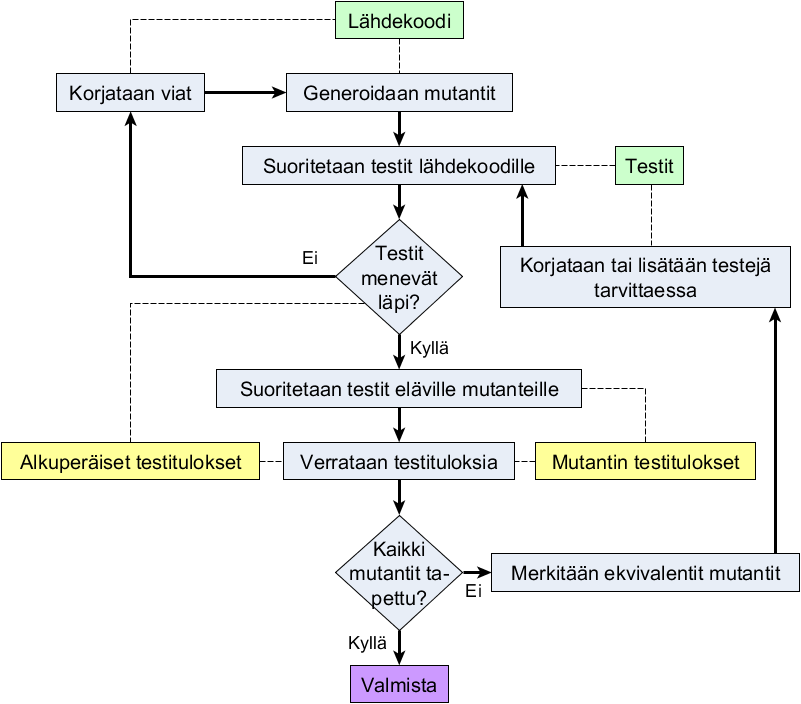
\includegraphics[width=\textwidth]{mutaatiotestausprosessi3}
	\caption{Perinteinen mutaatiotestausprosessi.}
	\label{figure:Mutaatiotestausprosessi}
\end{figure}

\subsection{Uusi mutaatiotestausprosessi}

Perinteiseen mutaatiotestausprosessiin sisältyy useita manuaalista työtä vaativia työvaiheita. Kuvassa \ref{figure:Mutaatiotestausprosessi} esitellyssä perinteisessä mutaatiotestausprosessissa manuaalista työtä vaativat työvaiheet ovat alkuperäisten testitulosten tarkastaminen, lähdekoodin vikojen korjaaminen, ekvivalenttien mutanttien merkitseminen ja uusien testien lisääminen tai olemassa olevien testien kehittäminen. 

Kuvan \ref{figure:Mutaatiotestausprosessi} kaaviosta nähdään, että mutaatiotestaus ei ole suoraviivainen prosessi, vaan prosessin suoritus saattaa haarautua ja palata takaisin jo suoritettuihin työvaiheisiin. Haarautumista tapahtuu esimerkiksi silloin, kun kaikkia mutantteja ei ole saatu tapettua tai testit eivät ole menneet läpi. Mutaatiotestausprosessiin muodostuu haarautumisesta johtuen silmukoita. Mutaatiotestausprosessin pääsilmukkaan kuuluu testien suoritus alkuperäiselle lähdekoodille, testitulosten tarkastus, testien suoritus mutanteille, testitulosten vertailu, ekvivalenttien mutanttien merkitseminen ja lopuksi uusien testien lisääminen tai olemassa olevien testien kehittäminen.

Jotta perinteistä mutaatiotestausprosessia voidaan tehostaa, manuaaliset työvaiheet on poistettava mutaatiotestausprosessin pääsilmukasta~\cite[s. 41]{Offutt:Untch:2001}. Tällöin perinteisen mutaatiotestausprosessin tilalle muodostuu uusi mutaatiotestausprosessi, jossa osa työläistä manuaalisista työvaiheista suoritetaan automaattisesti. Automatisoitavia työvaiheita ovat ekvivalenttien mutanttien tunnistaminen ja uusien testien generointi ja kehittäminen. Ainoaksi merkittäväksi manuaaliseksi työvaiheeksi uudessa prosessissa jää tarkistaa, ovatko alkuperäiselle lähdekoodille suoritetut testit menneet läpi.

Automatisoinnin lisäksi uudessa mutaatiotestausprosessissa työvaiheiden suoritusjärjestys muuttuu~\cite[s. 40]{Offutt:Untch:2001}. Manuaalinen testitulosten tarkastusvaihe siirretään pois mutaatiotestauksen pääsilmukasta suoritettavaksi pääsilmukasta poistuttaessa. Lisäksi ekvivalenttien mutanttien tunnistaminen suoritetaan ennen pääsilmukkaan siirtymistä. 

Perinteisessä mutaatiotestausprosessissa suoritus päättyy, kun mutaatiopistemäärä saavuttaa arvon 1. Uudessa mutaatiotestausprosessissa riittävä mutaatiopistemäärä määritellään pistemäärälle asetettavan raja-arvon avulla. Uudessa prosessissa pääsilmukan työvaiheita ovat testien generointi, suoritus ja kehittäminen. Testejä kehitetään poistamalla tehottomat testit eli testit, jotka eivät tappaneet yhtään mutanttia. Lisäksi pääsilmukassa tarkastetaan, onko mutaatiopistemäärän raja-arvo saavutettu. 

Työvaiheiden automatisointi ja niiden suoritusjärjestyksen muuttaminen tekevät uudesta mutaatiotestausprosessista tehokkaamman verrattuna perinteiseen mutaatiotestausprosessiin~\cite[s. 41]{Offutt:Untch:2001}. Kuvassa \ref{figure:UusiMutaatiotestausprosessi} on esitelty uusi mutaatiotestausprosessi. Automatisoidut työvaiheet on merkitty kuvaan oransseilla laatikoilla ja manuaaliset työvaiheet on merkitty sinisillä laatikoilla. Prosessissa käytettäviä resursseja kuvataan vihreillä ja keltaisilla laatikoilla.

\begin{figure}[H]
	\centering
		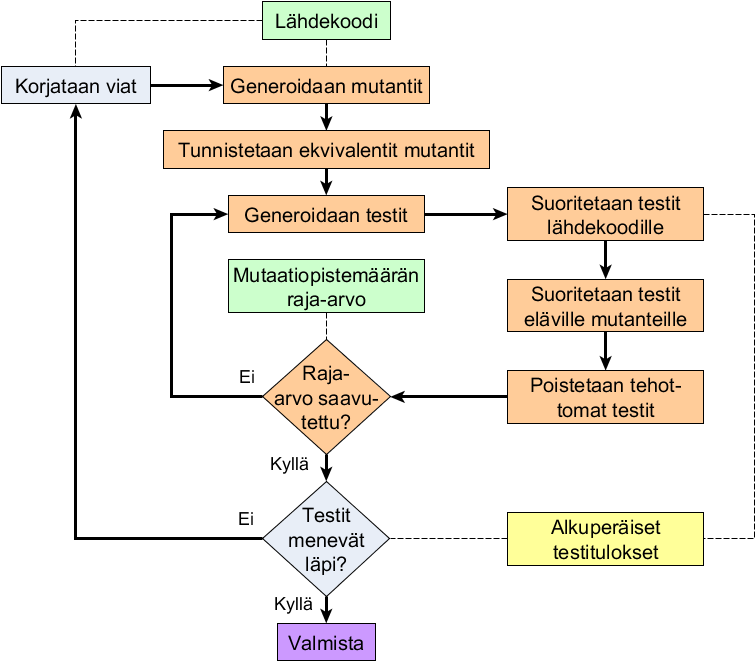
\includegraphics[width=\textwidth]{uusiprosessi}
	\caption{Uusi mutaatiotestausprosessi~\cite[s. 41]{Offutt:Untch:2001}.}
	\label{figure:UusiMutaatiotestausprosessi}
\end{figure}


\subsection{Mutaatio-operaattorit oliojärjestelmissä}

%Kappaleen estittelyteksti tähän. \textbf{Kuinka pitkä tämän on oltava?} 

%\subsection{Mutaatio-operaattorit}

Mutaatio-operaattorit ovat tärkeässä asemassa mutaatiotestauksessa, sillä mutaatiotestauksen tehokkuus riippuu siitä, minkälaisia vikoja mutaatio-operaattoreilla luodaan lähdekoodiin~\cite[s. 352]{Ma:Kwon:Offutt:2002}. Perinteisesti mutaatiotestausta on hyödynnetty proseduraalisessa ohjelmoinnissa, minkä vuoksi myös mutaatio-operaattorit on kehitetty tukemaan suurinta osaa proseduraalisten ohjelmointikielten piirteistä~\cite[s. 352]{Ma:Kwon:Offutt:2002}. 

Olioperustaisiin ohjelmointikieliin sisältyy kuitenkin uusia ominaisuuksia, joiden käytöstä aiheutuu erilaisia virheitä/vikoja verrattuna proseduraalisessa ohjelmoinnissa esiintyviin virheisiin/vikoihin. Uusien virheiden/vikojen ilmeneminen olio-ohjelmissa on johtanut uusien olioperustaisten mutaatio-operaattorien kehittämiseen.  

Olioperustaisten ohjelmien mutaatiotestaukseen käytettävää menetelmää kutsutaan \textit{luokkamutaatioksi}~\cite{Kim:Clark:McDermid:2000}. Luokkamutaatiomenetelmän kehittivät Sunwoo Kim, John Clark ja John McDermid Java-oh\-jel\-moin\-ti\-kie\-len käytöstä aiheutuvien vikojen pohjalta~\cite{Kim:Clark:McDermid:2000}. Heidän kehittämiensä \textit{luokkamutaatio-operaattorien} avulla mutaatiotestausmenetelmää voidaan soveltaa Java-ohjelmointikielellä toteutettuihin olioperustaisiin ohjelmiin.

Kimin, Clarkin ja McDermidin kehittämät luokkamutaatio-operaattorit ovat toimineet lähtökohtana myös muiden tutkijoiden luokkamutaatiotutkimuksessa ja uusien luokkamutaatio-operaattorien kehittämisessä. Yu Seung Ma, Yong Rae Kwon ja Jeff Offutt kehittivät vuonna 2002 Java-oh\-jel\-moin\-ti\-kiel\-tä varten joukon uusia luokkamutaatio-operaattoreita, jotka perustuivat aiemmin kehitettyihin operaattoreihin~\cite[s. 352]{Ma:Kwon:Offutt:2002}. Heidän tavoitteenaan oli parantaa ja kehittää olemassa olevia luokkamutaatio-operaattoreita, jotta luokkien välisten suhteiden testaaminen olisi mahdollista mutaatiotestauksella~\cite[s. 362]{Ma:Kwon:Offutt:2002}.

Taulukossa \ref{table:Mutaatio-operaattorit-taulukko} on listattu Man, Kwonin ja Offuttin kehittämät luok\-ka\-mu\-taa\-ti\-o-o\-pe\-raat\-to\-rit. Operaattorit on jaettu kuuteen ryhmään. Ryhmät perustuvat niihin olio-ohjelmointikielen piirteisiin, joita ryhmän operaattoreilla muunnetaan~\cite[s. 355]{Ma:Kwon:Offutt:2002}.

Mutaatio-operaattorien avulla kuvataan algoritmeja, joilla lähdekoodia muokataan mutantteja muodostettaessa. Esimerkiksi JSC-operaattori lisää ilmentymämuuttujiin \textit{static}-määreen tehden niistä luokkamuuttujia tai vastaavasti poistaa luokkamuuttujista \textit{static}-määreen tehden niistä ilmentymämuuttujia. JSC-operaattorin ja myös muiden Man, Kwonin ja Offuttin kehittämien luokkamutaatio-operaattorien nimet ja kuvaukset voi nähdä taulukosta \ref{table:Mutaatio-operaattorit-taulukko}. Taulukosta nähdään myös, mihin ryhmiin luokkamutaatio-operaattorit kuuluvat. Tarkemmat tiedot operaattorien toiminnasta löytyvät Man, Kwonin ja Offuttin artikkelista ''Inter-class mutation operators for Java''~\cite{Ma:Kwon:Offutt:2002}. 

\begin{table}[H]
\begin{spacing}{1.0}
	\begin{center}
		\centering
		\begin{tabulary}{1\textwidth}{|L|L|L|}
			\hline
			\textbf{Ryhmä} & \textbf{Operaattori} & \textbf{Kuvaus} \\
			\hline
			\parbox[t]{2cm}{Kapselointi} & AMC & Access modifier change \\
			\hline
			\multirow{8}{*}{\parbox[t]{2cm}{Perintä}} & IHD & Hiding variable deletion \\ \cline{2-3}
			& IHI & Hiding variable insertion \\ \cline{2-3}
			& IOD & Overriding method deletion \\ \cline{2-3}
			& IOP & \parbox[t]{7cm}{Overridden method calling position change} \\ \cline{2-3}
			& IOR & Overridden method rename \\ \cline{2-3}
			& ISK & \textit{super} keyword deletion \\ \cline{2-3}
			& IPC & \parbox[t]{7cm}{Explicit call of a parent's constructor deletion} \\
			\hline
			\multirow{7}{*}{\parbox[t]{2cm}{Polymor-\\fismi}} & PNC & \textit{new} method call with child class type \\ \cline{2-3}
			& PMD & \parbox[t]{7cm}{Member variable declaration with parent class type} \\ \cline{2-3}
			& PPD & \parbox[t]{7cm}{Parameter variable declaration with\\child class type}
\\ \cline{2-3}
			& PRV & \parbox[t]{7cm}{Reference assignment with other\\compatible type} \\
			\hline
			\multirow{4}{*}{\parbox[t]{2cm}{Metodin\\kuormi-\\tus}} & OMR & Overloading method contents change \\ \cline{2-3}
			& OMD & Overloading method deletion \\ \cline{2-3}
			& OAO & Argument order change \\ \cline{2-3}
			& OAN & Argument number change \\
			\hline 
			\multirow{4}{*}{\parbox[t]{2cm}{Javan\\erityis-\\piirteet}} & JTD & \textit{this} keyword deletion \\ \cline{2-3}
			& JSC & \textit{static} modifier change \\ \cline{2-3}
			& JID & Member variable initialization deletion \\ \cline{2-3}
			& JDC &  \parbox[t]{7cm}{Java-supported default constructor create} \\
			\hline
			\multirow{5}{*}{\parbox[t]{2cm}{Yleiset\\ohjelmoin-\\tivirheet}} & EOA & \parbox[t]{7cm}{Reference assignment and content assignment replacement} \\ \cline{2-3}
			& EOC & \parbox[t]{7cm}{Reference comparison and content comparison replacement} \\ \cline{2-3}
			& EAM & Accessor method change \\ \cline{2-3}
			& EMM & Modifier method change \\
			\hline
		\end{tabulary}
	\end{center}      
	\caption{Luokkamutaatio-operaattoreita Javalle~\cite{Ma:Kwon:Offutt:2002}.}
	\label{table:Mutaatio-operaattorit-taulukko}
\end{spacing}
\end{table}


%\subsection{Automatisoidut mutaatiotestausjärjestelmät}
%Mutaatiojärjestelmät opetuksessa: PIT. 
%Mutaatiojärjestelmä tutkimuksessa: MuJava.

\section{Mutaatiotestauksen haasteet}

Mutaatiotestausta voidaan käyttää ohjelmiston olemassa olevien testien kehittämiseen ja testien laadun parantamiseen. Mutaatiotestausmenetelmän käyttö ei ole kuitenkaan ongelmatonta. Mutaatiotestaukseen liittyy haasteita ja ratkaisemattomia ongelmia, jotka estävät menetelmän käyttämisen laaja-alaisesti osana testausprosessia~\cite[s. 652]{Jia:Harman:2011}.

Vaikka kaikkia mutaatiotestauksen ongelmia ei ole mahdollista ratkaista, mutaatiotestauksessa tapahtuneen edistyksen ansiosta ongelmien osittainen ratkaiseminen on kuitenkin mahdollista~\cite[s. 653]{Jia:Harman:2011}. Osittaisten ratkaisujen avulla mutaatiotestausprosessi on mahdollista automatisoida. 
%\textbf{Although it is impossible to completely solve these problems, with existing advances in mutation testing the process of mutation testing can be automated and the runtime can allow for reasonable scalability, as this survey will show.} 
Kuvassa \ref{figure:UusiMutaatiotestausprosessi} sivulla \pageref{figure:UusiMutaatiotestausprosessi} on esitelty uusi mutaatiotestausprosessi, jossa hyödynnetään työvaiheiden automatisointia. Uudessa mutaatiotestausprosessissa automatisoitujen työvaiheiden toteutuksessa voidaan käyttää menetelmiä, joiden avulla mutaatiotestauksen haasteita ja ongelmia on yritetty ratkaista.

%\textbf{Misi mutaatiotestaus ei ole päätynyt suureen suosioon/käyttöön? Valitaan muutama haaste ja esitellään niitä? Kerrotaan että myös muita haasteita, mutta ei esitellä niitä niin tarkasti?} HAASTEITA ON JAETTAVA TUTKIELMASSA OMIIN ALALUKUIHINSA. NYT TEHDÄÄN VAIN HAASTEITA VARTEN NS. "JOHDANTOKAPPALE" JONKA VOI TUTKIELMASSA JAKAA OMIKSI KAPPALEIKSEEN.

\subsection{Ekvivalentit mutantit}

Ekvivalenttien mutanttien tunnistaminen on yksi mutaatiotestaukseen liittyvistä ongelma-alueista. Ekvivalentit mutantit ovat mutantteja, jotka ovat toiminnaltaan samanlaisia kuin alkuperäinen ohjelma, mutta syntaktisesti erilaisia alkuperäisen ohjelman kanssa~\cite[s. 652]{Jia:Harman:2011}. Ekvivalentteja mutantteja muodostuu, kun alkuperäistä lähdekoodia käsitellään mutaatio-operaattoreilla. 

Esimerkissä 1 on esitelty esimerkki IHI-operaattorin tuottamasta ekvivalentista mutantista. Taulukossa \ref{table:Mutaatio-operaattorit-taulukko} sivulla \pageref{table:Mutaatio-operaattorit-taulukko} esitelty mutaatio-operaattori IHI lisää aliluokkaan kentän, joka peittää yliluokalta perityn kentän. Jos peittävä kentä on yliluokassa määritelty yksityiseksi, kaikki IHI-operaattorilla tuotetut mutantit ovat ekvivalentteja mutantteja~\cite[s. 80]{Offutt:Ma:Kwon:2006:MuClassLevel}. Esimerkissä 1 IHI-operaattorilla on muodostettu mutantti, jossa \texttt{Kauppa}-luokan aliluokaan \texttt{Elainkauppa} on lisätty peittävä kenttä \texttt{osoite}. \texttt{Elainkauppa}-luokassa yliluokan \texttt{osoite}-muuttuja saadaan käyttöön yliluokan metodilla \texttt{getOsoite()}. Peittävän kentän \texttt{osoite} lisääminen ei siis muuta luokan \texttt{Elainkauppa} toimintaa, joten kyseessä on ekvivalentti mutantti. 

\vspace{1\baselineskip}\noindent\textbf{Esimerkki 1}
\begin{lstlisting} 
public class Kauppa {
	private String osoite;
	public void setOsoite(String uusiOsoite){
		this.osoite = uusiOsoite;
	};
	public String getOsoite(){
		return this.osoite;
	};
};

public class Elainkauppa extends Kauppa {
	private String osoite; //IHI operaattorin lisaama muuttuja
	private String erikoisala = "kissanruuat";
	public String toString(){
		return "Liikkeen osoite on " + getOsoite() +
		        " ja sen erikoisalana on " + this.erikoisala;
	};
};
\end{lstlisting}

\vspace{1\baselineskip}On todistettu, että ekvivalenttien mutanttien tunnistaminen \textbf{(algoritmisesti)} yleisessä tapauksessa on ratkaisematon ongelma~\cite[s. 79]{Offutt:Ma:Kwon:2006:MuClassLevel}. Ekvivalenttien mutanttien tunnistamiseksi on kuitenkin kehitetty heuristiikkoja, joiden avulla ongelma voidaan ratkaista osittain. Tunnistamisongelma on herättänyt runsaasti teoreettista kiinnostusta, ja mahdollisia tunnistamistekniikoita on tutkittu paljon~\cite[s. 657]{Jia:Harman:2011}. 

Yksi vaihtoehto ekvivalenttien mutanttien tunnistamisongelman ratkaisemiseksi on estää ekvivalenttien mutanttien syntyminen mutanttien generointivaiheessa~\cite[s. 80]{Offutt:Ma:Kwon:2006:MuClassLevel}. Useita menetelmiä on myös kehitetty ekvivalenttien mutanttien tunnistamiseksi mutanttien generoinnin jälkeen~\cite[s. 79]{Offutt:Ma:Kwon:2006:MuClassLevel}~\cite[s. 657]{Jia:Harman:2011}.

Heuristiikkojen avulla voidaan tunnistaa vain osa ekvivalenteista mutanteista. Jos kaikki ekvivalentit mutantit halutaan tunnistaa, tunnistaminen on suoritettava manuaalisesti tutkimalla mutanttia ja vertaamalla mutantin toimintaa alkuperäisen ohjelmiston toimintaan. Ekvivalenttien mutanttien tunnistaminen manuaalisesti lisää kuitenkin mutaatiotestaukseen vaadittavaa työmäärää.

\subsection{Tehokkuusongelmat}

Tehokkuuteen liittyvät ongelmat ovat toinen mutaatiotestauksen ongelma-alueista. Tehokkuusongelmia esiintyy erityisesti silloin, kun jokaisen mutantin kohdalla suoritetaan kaikki ohjelmistoa varten tehdyt testit~\cite[s. 652]{Jia:Harman:2011}. Testien suoritus jokaisen mutantin kohdalla hidastaa mutaatiotestausprosessia ja vaatii paljon laskentatehoa. Tehokkuusongelman ratkaisemiseksi on kuitenkin esitetty useita ratkaisuehdotuksia~\cite[s. 653]{Jia:Harman:2011}. Ratkaisuehdotuksia ovat esimerkiksi generoitujen mutanttien määrän vähentäminen ja mutanttien ja testien suorituskustannusten pienentäminen.

Ratkaisuehdotukset mutaatiotestauksen vaatiman laskentatehon \textbf{(computational cost)} vähentämiseksi on jaettu kolmeen osa-alueeseen~\cite[s. 37]{Offutt:Untch:2001}. Osa-alueisiin sisältyy menetelmiä, joiden avulla mutaatiotestauksen laskentakustannuksia pienennetään. Mutaatiotestauksessa laskentaa voidaan tehostaa tekemällä mutaatiotestausta \textit{viisaammin} (\textit{do smarter}), \textit{nopeammin} (\textit{do faster}) ja \textit{pienemmällä mutanttimäärällä} (\textit{do fewer}) kuin aiemmin~\cite[s. 37]{Offutt:Untch:2001}.

Yksi menetelmä tehdä mutaatiotestausta viisaammin on hajauttaa laskentatyö usealle laitteelle~\cite[s. 38]{Offutt:Untch:2001}. Koska mutantit ovat riippumattomia toisistaan, mutanttien suorituksen hajauttamiseen ei liity suuria kommunikointikustannuksia. Toinen esimerkki viisaammasta mutaatiostestauksesta on käyttää \textit{heikkoa mutaatiota} (\textit{weak mutation})~\cite[s. 37]{Offutt:Untch:2001} \textit{vahvan mutaation} (\textit{strong mutation})~\cite[s. 655]{Jia:Harman:2011} sijasta. Vahvassa mutaatiossa mutanttien suorituksesta saatuja tulosteita verrataan alkuperäisen ohjelmiston tulosteisiin vasta, kun mutantin suoritus on päättynyt kokonaan~\cite[s. 37]{Offutt:Untch:2001}. Heikossa mutaatiossa alkuperäisen ohjelman \textbf{sisäistä tilaa internal state} verrataan mutantin sisäiseen tilaan, kun muunnettu lähdekoodin kohta on suoritettu mutanttia testattaessa.

Kun mutaatiotestausta yritetään tehdä nopeammin, etsitään tapoja generoida ja suorittaa mutantteja mahdollisimman nopeasti~\cite[s. 37]{Offutt:Untch:2001}. Yksi vaihtoehto mutaatiotestauksen nopeuttamiseksi on käyttää \textit{MSG-metodia} (\textit{Mutant Schema Generation method}) mutaatiotestauksessa~\cite[s. 38]{Offutt:Untch:2001}. MSG-metodissa kaikista mutanteista muodostetaan metamutantti, johon sisällytetään kaikki lähdekoodista generoidut mutantit. Metamutantin generoinnin jälkeen metamutantti käännetään samalla kääntäjällä, jota käytetään alkuperäisen lähdekoodin kääntämiseen. Metamutantti \textbf{runs at compile-speeds/ is executed in the same operational environment at com\-pi\-led-prog\-ram speeds} voidaan suorittaa yhtä nopeasti kuin normaali käännetty ohjelma. Suorituksen aikana metamutantti voidaan dynaamisesti muuttaa edustamaan mitä tahansa alkuperäisestä lähdekoodista muodostettua mutanttia~\cite[s. 105]{Ma:Offutt:Kwon:2005:MuAutomated}.

Laskentaa voidaan tehostaa mutaatiotestauksessa karsimalla mutanttien lukumäärää. Mutanttien määrää vähennettäessä etsitään tapoja pienentää mutanttien kappalemäärää menettämättä kuitenkaan liikaa tietoa testien laadusta~\cite[s. 37]{Offutt:Untch:2001}. Yksi vaihtoehto suoritettavien mutanttien lukumäärän pienentämiseksi on valita generoiduista mutanteista sattumanvaraisesti mutanttien osajoukko käytettäväksi mutaatiotestauksessa. Toinen esimerkki mutanttien määrän vähentämiseksi on jättää käyttämättä kaikkia mutaatio-operaattoreita mutantteja generoitaessa. Tätä menetelmää, jossa mutaatio-operaattoreista valitaan vain osajoukko käytettäväksi mutanttien generoinnissa kutsutaan \textit{valikoivaksi mutaatioksi} (\textit{selective mutation})~\cite[s. 37]{Offutt:Untch:2001}.

\subsection{Manuaalinen työ}

Kolmas mutaatiotestauksen ongelma-alue liittyy perinteiseen mutaatiotestausprosessiin sisältyvään manuaaliseen työhön. Perinteisessä mutaatiotestausprosessissa useaan prosessin työvaiheeseen sisältyy manuaalista työtä. Kuvassa \ref{figure:Mutaatiotestausprosessi} sivulla \pageref{figure:Mutaatiotestausprosessi} on esitelty perinteinen mutaatiotestausprosessi. Kuvassa olevaan kaavioon on merkitty työvaihe, jossa alkuperäisten testien suorituksen jälkeen tarkastetaan, ovatko testit menneet läpi. 

Testien läpimenotarkastus on usein testausprosessin työläin osa~\cite[s. 653]{Jia:Harman:2011}. Tämä ongelma ei liity pelkästään mutaatiotestaukseen vaan ongelma ilmenee myös muissa testausmenetelmissä. Jos testien odotettuja tuloksia varten ei ole olemassa määrittelyä, kuten esimerkkitapauksia (\textit{assertion}), ihmisen on toimittava testioraakkelina ja päätettävä, toimiiko ohjelma oikein~\cite[s. 519]{Barr:Harman:McMinn:Shahbaz:Yoo:2015}. Tällaisessa tapauksessa ihminen toimii \textit{ihmisoraakkelina} (\textit{human oracle}). Koska mutaatiotestauksessa suoritetaan usein paljon testejä, testauksen tulosten tarkastamiseen vaadittava työmäärä kasvaa~\cite[s. 653]{Jia:Harman:2011}.

Uusien, mutantteja tappavien testien kehittäminen on myös yksi perinteisen mutaatiotestausprosessin työläistä manuaalisista työvaiheista~\cite[s. 39]{Offutt:Untch:2001}. Mutaatiotestauksessa tavoitteena on kehittää testejä, jotka tappavat mahdollisimman paljon mutantteja. Manuaalisesti tällaisten testien kehittäminen on työlästä. Lisäksi sopivien syötteiden löytäminen testejä varten on yksi vaikeimmista testauksen vaiheista~\cite[s. 39]{Offutt:Untch:2001}. Testien automaattista generointia varten on kuitenkin kehitetty menetelmiä, joiden avulla testien generointi voidaan mutaatiotestausprosessissa automatisoida osittain~\cite[s. 39]{Offutt:Untch:2001}.


%__________________________________________________________

%\section{Miten mutaatiotestaus auttaa testien laadun parantamisessa?}

%\subsection{Miksi mutaatiotestausta tulisi käyttää, vaikka se on raskasta ja työlästä?}

%\subsection{Miltä tulevaisuus näyttää, tuleeko käyttö lisääntymään vai jääkö mutaatiotestaus unohduksiin/pienen piirin harrastukseksi?}


\section{Yhteenveto}

Olioperustaisen ohjelmoinnin mukana tulevien uusien haasteiden kohtaaminen vaatii muutoksia myös ohjelmistojen testausmenetelmiin. Sekä perinteisiä olemassa olevia että uusia testausmenetelmiä kehitetään, jotta olio-ohjelmia voidaan testata kattavasti ja laadukkaasti. 

Perinteisessä ohjelmistotestauksessa keskitytään ohjelmiston toiminnallisuuden testaamiseen ja vikojen etsimiseen ohjelmistosta. Perinteiseen ohjelmistotestaukseen liittyy kuitenkin haasteita, jotka aiheuttavat testaukseen epävarmuutta. Yksi haasteista on määrittää, ovatko testauksessa käytettävät testit ja testausjärjestelmä riittävän luotettavia, jotta niiden avulla ohjelmistoa voidaan testata laadukkaasti.

Mutaatiotestaus on virheperustainen testausmenetelmä, joka tarjoaa ratkaisun testien laadun määrittämiseen liittyvään haasteeseen. Mutaatiotestauksen avulla voidaan mitata ohjelmistoa varten tehtyjen testien kykyä havaita ohjelmistossa esiintyviä vikoja. Mutaatiotestausmenetelmän avulla on siis mahdollista kehittää olemassa olevia testejä ja parantaa testien luotettavuutta.

Mutaatiotestauksen käyttö yleisesti osana testausprosessia on vähäistä mutaatiotestaukseen liittyvien ratkaisemattomien ongelmien takia. Mutaatiotestausta on kuitenkin tutkittu paljon. Tutkimuksen avulla voi olla mahdollista löytää ratkaisuja mutaatiotestausta vaivaaviin ongelmiin, jotta mutaatiotestauksen laaja-alainen käyttö voisi tulevaisuudessa olla mahdollista.

%Tällä (yksikkö)testauksen tasolla testien suunnittelussa voidaan käyttää ohjelman sisäiseen rakenteeseen perustuvaa suunnittelumallia, jota kutsutaan \textit{white box -testaukseksi} (\textit{white box testing}). Tässä mallissa ohjelmiston lähdekoodia käytetään apuna testien valmistamisessa~\cite[s. 52]{Binder:1999}.

%Tämän tason testien suunnittelustrategiana voidaan käyttää ohjelmiston ulkoisen toiminnallisuuden analysointia. Tällaista testausstrategiaa kutsutaan \textit{black box -testaukseksi} (\textit{black box testing}) tai \textit{funktionaaliseksi testaukseksi} (\textit{functional testing})~\cite[s. 52]{Binder:1999}. Kuitenkin sekä white box - että black box -testausta voidaan käyttää kaikilla testauksen tasoilla testien suunnittelun apuna. 

%\section{Miten saa evaluointia/analyysiä? Mihin lukuihin se sopii?}

%\textbf{Mihin kohtiin evaluointi ja analyysi sopivat, jotta tästä ei tule mutaatiotestauksen/testauksen oppikirjaa? Miten sitä tehdään? Vertailemalla, ennustamalla tulevaa, jotakin muuta?}

%Evaluointi ja analyysi ovat jossain määrin vähemmän sisältäviä kuin voisi kuvitella. Analyysi esim. on pääasiassa vaikka asioiden vertailua (koska omaa tutkimusta ei tehdä). Evaluointi taas on esimerkiksi tiedon rajaamista ja esittämistä yhdisteltynä toisiin tietoihin. Ts. olet joutunut itse keräämään tiedon ja rajaamaan sen sopivaksi joukoksi infoa tätä tutkielmaa varten. Siitä muodostuu evaluointi osa.


% --- References ---
%
% bibtex is used to generate the bibliography. The babplain style
% will generate numeric references (e.g. [1]) appropriate for theoretical
% computer science. If you need alphanumeric references (e.g [Tur90]), use
%
\newpage
\bibliographystyle{babalpha-lf}
%
% instead.

%\bibliographystyle{babplain-lf}
\bibliography{references-fi}


% --- Appendices ---

% uncomment the following

% \newpage
% \appendix
% 
% \section{Esimerkkiliite}

\end{document}
